\renewcommand{\floatpagefraction}{0.1}

\begin{figure}[t!]
	\begin{center}
	\includesvg[width=\textwidth]{figures/papers_over_years}
	\caption{Numbers of papers published per year with topic "augmented reality" and "education" as of 1 October 2020.}
	\label{fig:pappublbg}
    \end{center}
\end{figure}

\clearpage
\newpage

\begin{figure}[t!]	
	\begin{center}
	%\includesvg[width=0.48\textwidth]{figures/prisma}
	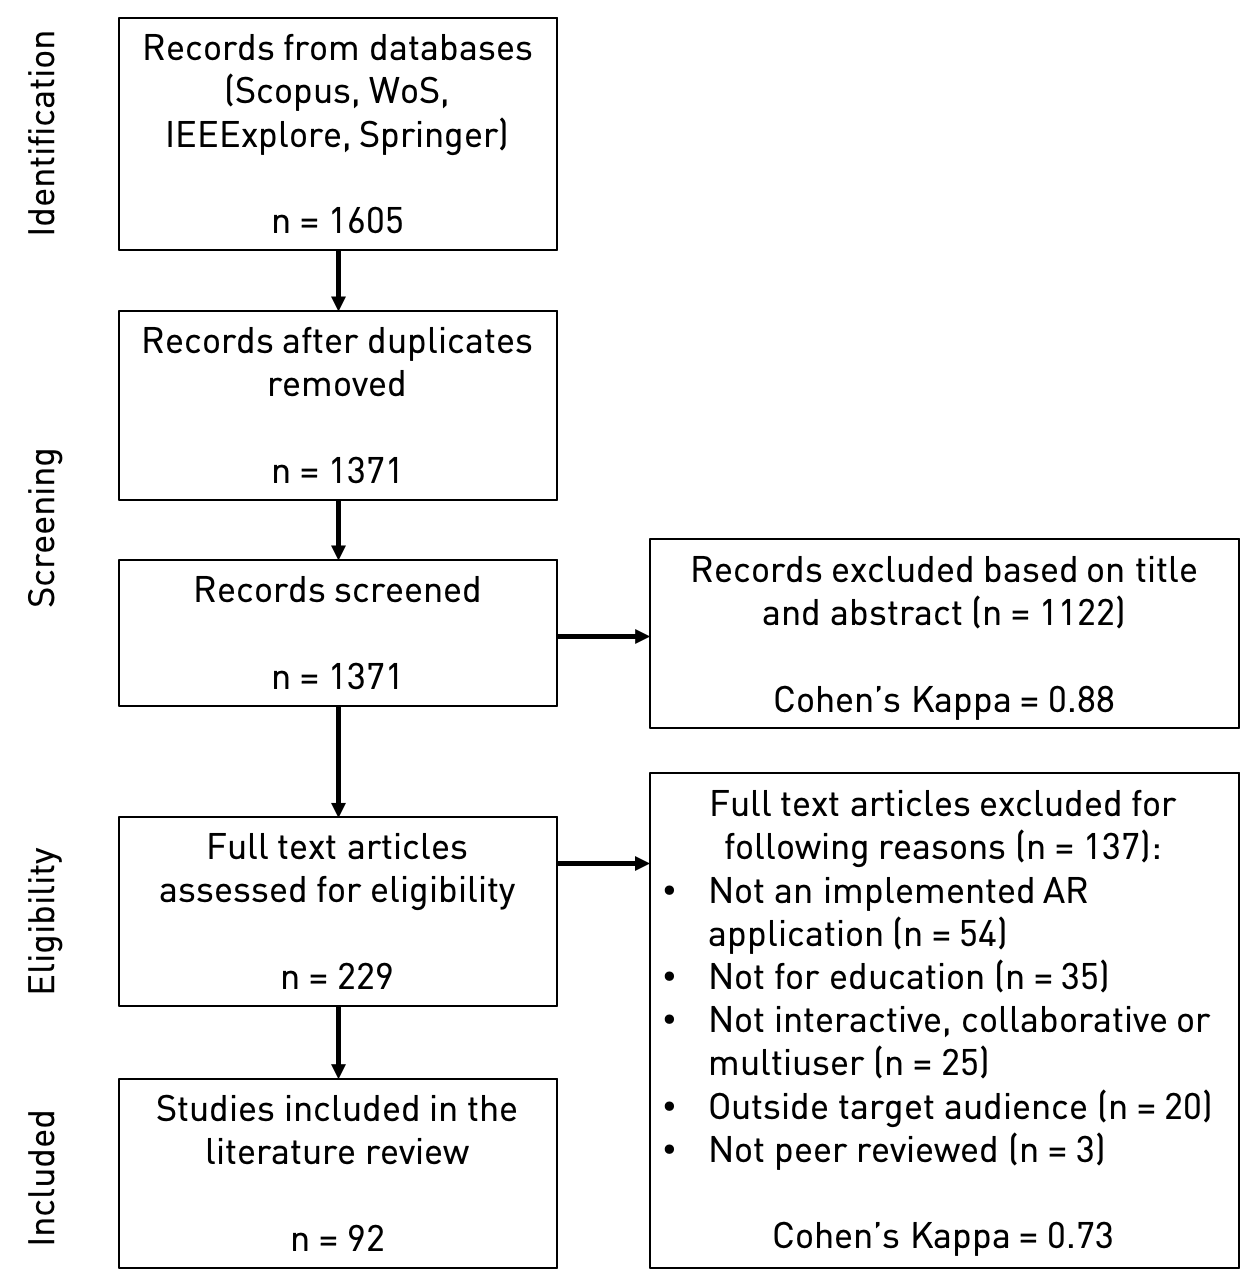
\includegraphics[width=\textwidth]{figures/prisma.png}
	\caption{Prisma flowchart of the search protocol.}
	\label{fig:flowchart}
    \end{center}
\end{figure}

\clearpage
\newpage

\begin{figure}[t!]	
	\begin{center}
	\includesvg[width=\textwidth]{figures/subjects}
	\caption{Subjects covered in the studies analysed.}
	\label{fig:subjects}
    \end{center}
\end{figure}

\clearpage
\newpage

\begin{figure}[t!]	
	\begin{center}
	\includesvg[width=\textwidth]{figures/AR_technology}
	\caption{Different types of AR used in the studies analysed.}
	\label{fig:artech}
    \end{center}
\end{figure}

\clearpage
\newpage

\begin{figure}[t!]	
	\begin{center}
	\includesvg[width=\textwidth]{figures/Hardware_supported}
	\caption{Device types supported by the AR applications.}
	\label{fig:hardware}
    \end{center}
\end{figure}

\clearpage
\newpage

\begin{figure}[t!]	
	\begin{center}
	\includesvg[width=\textwidth]{figures/Software_used}
	\caption{Software used to develop AR applications.}
	\label{fig:software}
    \end{center}
\end{figure}

\clearpage
\newpage

\begin{figure}[t!]	
	\begin{center}
	\includesvg[width=\textwidth]{figures/hist_testers}
	\caption{Histogram of the participant in user tests across different studies (grey) and its smooth density estimate (black).}
	\label{fig:testers}
    \end{center}
\end{figure}

\clearpage
\newpage